\documentclass[aspectratio=169]{beamer}

\usepackage{ccicons}
\usepackage{fontspec}
\usepackage{listings}
\usepackage{tikz}
\usepackage{svg}

\definecolor{uclablue}{RGB}{39,116,174}
\definecolor{uclagold}{RGB}{255,179,0}

\definecolor{ubcorange}{RGB}{158, 66, 37}

\definecolor{cugold}{RGB}{207, 184, 124}
\definecolor{cudarkgray}{RGB}{86, 90, 92}

\definecolor{solarizedred}{RGB}{220, 50, 47}
\definecolor{solarizedblue}{RGB}{38, 139, 210}
\definecolor{solarizedgreen}{RGB}{133, 153, 0}
\definecolor{solarizedpurple}{RGB}{108, 113, 196}
\definecolor{solarizedmagenta}{RGB}{211, 54, 130}

\definecolor{pantone655}{RGB}{0, 42, 92}
\definecolor{pantone7453}{RGB}{123, 164, 217}
\definecolor{pantone633}{RGB}{0, 139, 176}
\definecolor{pantone7492}{RGB}{218, 229, 205}

\colorlet{primarycolor}{pantone655}
\colorlet{secondarycolor}{pantone7453}


\usetikzlibrary{
  arrows,
  arrows.meta,
  automata,
  backgrounds,
  calc,
  chains,
  decorations.pathreplacing,
  fit,
  intersections,
  matrix,
  overlay-beamer-styles,
  positioning,
  shapes,
  shapes.multipart,
  tikzmark,
}
\usetikzmarklibrary{listings}

\hypersetup{
  colorlinks=true,
  urlcolor=cudarkgray,
}

\setbeamercolor{frametitle}{fg=primarycolor}
\setbeamercolor{structure}{fg=primarycolor}
\setbeamercolor{enumerate item}{fg=black}
\setbeamercolor{itemize item}{fg=black}
\setbeamercolor{itemize subitem}{fg=black}

\setbeamersize{text margin left=26.6mm}
\addtolength{\headsep}{2mm}

\setbeamertemplate{navigation symbols}{}
\setbeamertemplate{headline}{}
\setbeamertemplate{footline}{}
\setbeamertemplate{itemize item}{\color{black}}
\setbeamertemplate{itemize items}[circle]

\setbeamertemplate{footline}{
  \begin{tikzpicture}[remember picture,
                      overlay,
                      shift={(current page.south west)}]
    \node [black!50, inner sep=2mm, anchor=south east]
          at (current page.south east) {\footnotesize \insertframenumber};
  \end{tikzpicture}
}

\setsansfont{Inter}[Scale=MatchLowercase]
\setmonofont{Hack}[Scale=MatchLowercase]

\makeatletter
\newcommand\version[1]{\renewcommand\@version{#1}}
\newcommand\@version{}
\def\insertversion{\@version}

\newcommand\lecturenumber[1]{\renewcommand\@lecturenumber{#1}}
\newcommand\@lecturenumber{}
\def\insertlecturenumber{\@lecturenumber}
\makeatother

\setbeamertemplate{title page}
{
  \begin{tikzpicture}[remember picture,
                      overlay,
                      shift={(current page.south west)},
                      background rectangle/.style={fill=pantone655},
                      show background rectangle]
    \node [anchor=west, align=left, inner sep=0, text=white]
          (lecturenumber) at (\paperwidth / 6, \paperheight * 3 / 4)
          {\Large Lecture \insertlecturenumber};
    \node [inner sep=0, align=left, text=white, node distance=0,
          above left=of lecturenumber, anchor=south west, yshift=2mm]
          {\Large ECE 344: Operating Systems};
    \node (title) [inner sep=0, anchor=west, align=left, text=white,
                   text width=30em]
          at (\paperwidth / 6, \paperheight / 2)
          {{\bfseries \Huge \inserttitle{}}};
    \node [inner sep=0, align=right, text=white, node distance=0,
          below right=of title, anchor=north east, yshift=-1mm]
          {{\footnotesize \ttfamily \insertversion}};
    \node [inner sep=0, text=white, align=left, anchor=west]
          (author) at (\paperwidth / 6, \paperheight / 4)
          {\insertauthor};
    \node [text=white, inner sep=0, align=left, node distance=0,
           below left=of author, anchor=north west, yshift=-2mm]
          {\insertdate};
    \node [align=right, anchor=south east, inner sep=2mm, text=white]
          (license) at (\paperwidth, 0)
          {\footnotesize This  work is licensed under a
           \href{http://creativecommons.org/licenses/by-sa/4.0/}
                {\color{pantone7453} Creative Commons Attribution-ShareAlike 4.0
                 International License}};
    \node [text=white, inner sep=0, align=right, node distance=0,
           above right=of license, anchor=south east, xshift=-2mm]
          {\Large \ccbysa};
  \end{tikzpicture}
}

\tikzset{
  >=Straight Barb[],
  shorten >=1pt,
  initial text=,
}

\lstset{
  basicstyle=\footnotesize\ttfamily,
  language=C,
  escapechar=@,
  commentstyle=\color{black!50},
}


\lecturenumber{21}
\title{Page Replacement}
\version{1.0.0}
\author{Jon Eyolfson}
\date{October 31, 2022}

\tikzset{swapin/.style args = {(#1,#2)}{%
    row #1 column #2/.style={nodes={text=red}}}}

\begin{document}
  \begin{frame}[plain, noframenumbering]
    \titlepage
  \end{frame}

  \begin{frame}{Computer Memory Hierarchy is a Trade-off of Capacity and Speed}
    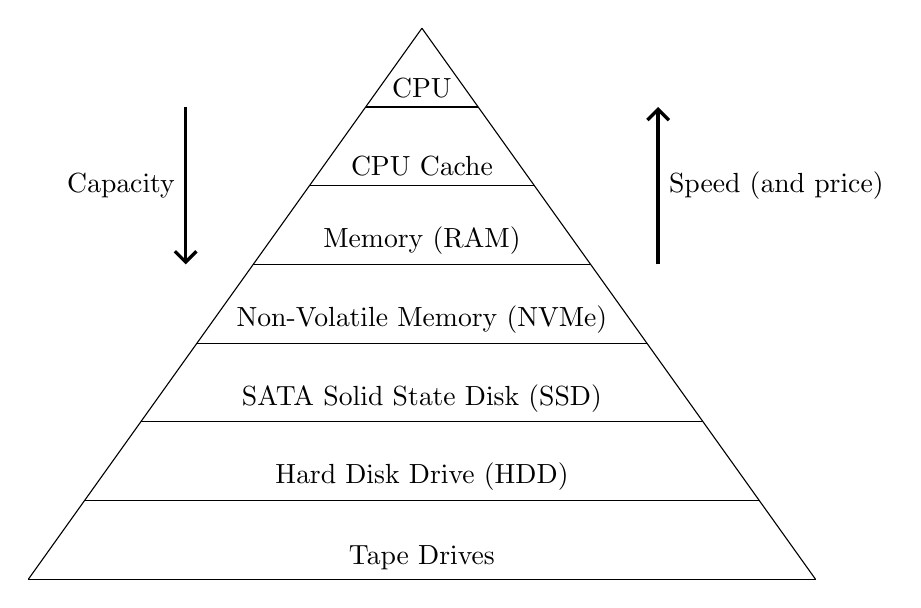
\begin{tikzpicture}[shorten >=0pt]
      \coordinate (A) at (-5,0) {};
      \coordinate (B) at ( 5,0) {};
      \coordinate (C) at (0,7) {};
      \draw[name path=AC] (A) -- (C);
      \draw[name path=BC] (B) -- (C);
      \foreach \y/\A in {
        0/Tape Drives,
        1/Hard Disk Drive (HDD),
        2/SATA Solid State Disk (SSD),
        3/Non-Volatile Memory (NVMe),
        4/Memory (RAM),
        5/CPU Cache,
        6/CPU
      } {
        \draw ($(A)!\y/7!(C)$) -- ($(B)!\y/7!(C)$)
          node[midway,above] {\A};
      }

      \draw [->, very thick] (-3,6) -- (-3,4) node[midway, left] {Capacity};
      \draw [->, very thick] (3,4) -- (3,6) node[midway, right] {Speed (and price)};
    \end{tikzpicture}
  \end{frame}

  \begin{frame}
    \frametitle{We Want to Hide the Hierarchy from the User}

    Each level wants to pretend it has the speed of the layer above it

    \hspace{2em} and the capacity of the layer below it

    \vspace{2em}

    The memory used by all the processes my exceed the amount of physical memory

    \hspace{2em} Not all of them may be in use at the same time

    \vspace{2em}

    Only keep referenced pages in memory, put others on disk

    \hspace{2em} Swap pages back to memory when they're needed
  \end{frame}

  \begin{frame}
    \frametitle{Page Replacement Algorithms}

    Optimal

    \hspace{2em} Replace the page that won't be used for the longest

    \vspace{2em}

    Random

    \hspace{2em} Replace a random page

    \vspace{2em}

    First-in First-out (FIFO)

    \hspace{2em} Replace the oldest page first
    
    \vspace{2em}

    Least Recently Used (LRU)

    \hspace{2em} Replace the page that hasn't been used in the longest time
  \end{frame}

  \begin{frame}
    \frametitle{Page Replacement Evaluation}

    Assume our physical memory can only hold 4 pages, and we access the following:

    \hspace{2em} 1 2 3 4 1 2 5 1 2 3 4 5 (all of the pages are initially on disk)

    \vspace{2em}

    We'll use this for a bunch of examples during this lecture

    \hspace{2em} We want the fewest number of page faults

    \vspace{2em}

    For every example we'll find the number of page faults
  \end{frame}

  \begin{frame}[fragile]
    \frametitle{Optimal Example}

    Assume our physical memory can only hold 4 pages, and we access the following:

    \hspace{2em} 1 2 3 4 1 2 5 1 2 3 4 5 (all of the pages are initially on disk)

    \begin{center}
      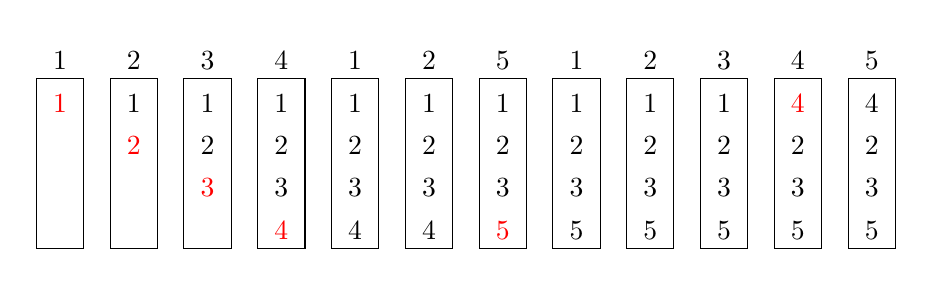
\begin{tikzpicture}[
        every node/.style={
          align=center,
          text height=2ex,
          text width=1em
        },
        swapin/.list={
          (2,1),
          (3,2),
          (4,3),
          (5,4),
          (5,7),
          (2,11)
        },
      ]
        \matrix (m) [
          matrix of nodes,
          nodes in empty cells,
          column sep=1em,
          column 2/.style={visible on=<2->},
          column 3/.style={visible on=<3->},
          column 4/.style={visible on=<4->},
          column 5/.style={visible on=<5->},
          column 6/.style={visible on=<6->},
          column 7/.style={visible on=<7->},
          column 8/.style={visible on=<8->},
          column 9/.style={visible on=<9->},
          column 10/.style={visible on=<10->},
          column 11/.style={visible on=<11->},
          column 12/.style={visible on=<12->},
        ] {
          1 & 2 & 3 & 4 & 1 & 2 & 5 & 1 & 2 & 3 & 4 & 5 \\
          1 & 1 & 1 & 1 & 1 & 1 & 1 & 1 & 1 & 1 & 4 & 4 \\
            & 2 & 2 & 2 & 2 & 2 & 2 & 2 & 2 & 2 & 2 & 2 \\
            &   & 3 & 3 & 3 & 3 & 3 & 3 & 3 & 3 & 3 & 3 \\
            &   &   & 4 & 4 & 4 & 5 & 5 & 5 & 5 & 5 & 5 \\
        };
        \draw (m-2-1.north west) rectangle (m-5-1.south east);
        \draw (m-2-2.north west) rectangle (m-5-2.south east);
        \draw (m-2-3.north west) rectangle (m-5-3.south east);
        \draw (m-2-4.north west) rectangle (m-5-4.south east);
        \draw (m-2-5.north west) rectangle (m-5-5.south east);
        \draw (m-2-6.north west) rectangle (m-5-6.south east);
        \draw (m-2-7.north west) rectangle (m-5-7.south east);
        \draw (m-2-8.north west) rectangle (m-5-8.south east);
        \draw (m-2-9.north west) rectangle (m-5-9.south east);
        \draw (m-2-10.north west) rectangle (m-5-10.south east);
        \draw (m-2-11.north west) rectangle (m-5-11.south east);
        \draw (m-2-12.north west) rectangle (m-5-12.south east);
      \end{tikzpicture}
    \end{center}

    \begin{flushright}
      \onslide<13->{6 page faults}
    \end{flushright}
  \end{frame}

  \begin{frame}[fragile]
    \frametitle{FIFO Example}

    Assume our physical memory can only hold 4 pages, and we access the following:

    \hspace{2em} 1 2 3 4 1 2 5 1 2 3 4 5 (all of the pages are initially on disk)

    \begin{center}
      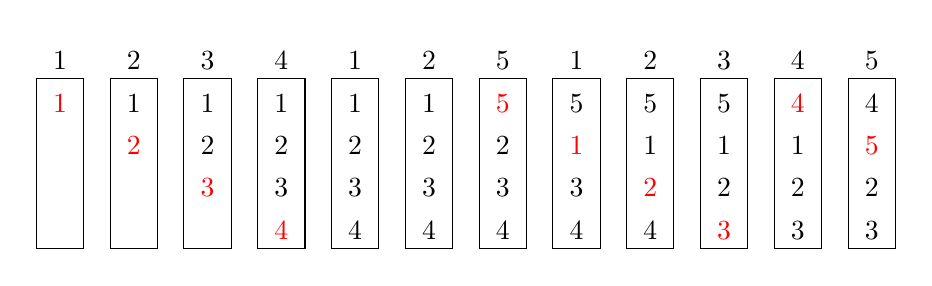
\begin{tikzpicture}[
        every node/.style={
          align=center,
          text height=2ex,
          text width=1em
        },
        swapin/.list={
          (2,1),
          (3,2),
          (4,3),
          (5,4),
          (2,7),
          (3,8),
          (4,9),
          (5,10),
          (2,11),
          (3,12)
        },
      ]
        \matrix (m) [
          matrix of nodes,
          nodes in empty cells,
          column sep=1em,
          column 2/.style={visible on=<2->},
          column 3/.style={visible on=<3->},
          column 4/.style={visible on=<4->},
          column 5/.style={visible on=<5->},
          column 6/.style={visible on=<6->},
          column 7/.style={visible on=<7->},
          column 8/.style={visible on=<8->},
          column 9/.style={visible on=<9->},
          column 10/.style={visible on=<10->},
          column 11/.style={visible on=<11->},
          column 12/.style={visible on=<12->},
        ] {
          1 & 2 & 3 & 4 & 1 & 2 & 5 & 1 & 2 & 3 & 4 & 5 \\
          1 & 1 & 1 & 1 & 1 & 1 & 5 & 5 & 5 & 5 & 4 & 4 \\
            & 2 & 2 & 2 & 2 & 2 & 2 & 1 & 1 & 1 & 1 & 5 \\
            &   & 3 & 3 & 3 & 3 & 3 & 3 & 2 & 2 & 2 & 2 \\
            &   &   & 4 & 4 & 4 & 4 & 4 & 4 & 3 & 3 & 3 \\
        };
        \draw (m-2-1.north west) rectangle (m-5-1.south east);
        \draw (m-2-2.north west) rectangle (m-5-2.south east);
        \draw (m-2-3.north west) rectangle (m-5-3.south east);
        \draw (m-2-4.north west) rectangle (m-5-4.south east);
        \draw (m-2-5.north west) rectangle (m-5-5.south east);
        \draw (m-2-6.north west) rectangle (m-5-6.south east);
        \draw (m-2-7.north west) rectangle (m-5-7.south east);
        \draw (m-2-8.north west) rectangle (m-5-8.south east);
        \draw (m-2-9.north west) rectangle (m-5-9.south east);
        \draw (m-2-10.north west) rectangle (m-5-10.south east);
        \draw (m-2-11.north west) rectangle (m-5-11.south east);
        \draw (m-2-12.north west) rectangle (m-5-12.south east);
      \end{tikzpicture}
    \end{center}

    \begin{flushright}
      \onslide<13->{10 page faults}
    \end{flushright}
  \end{frame}

  \begin{frame}[fragile]
    \frametitle{FIFO Example (3 Page Frames)}

    Assume our physical memory can only hold \textbf{3} pages, and we access the following:

    \hspace{2em} 1 2 3 4 1 2 5 1 2 3 4 5 (all of the pages are initially on disk)

    \begin{center}
      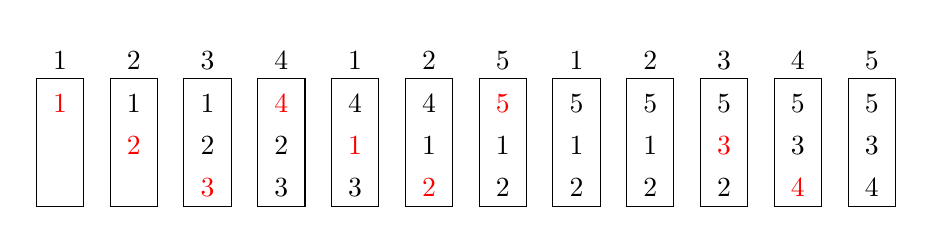
\begin{tikzpicture}[
        every node/.style={
          align=center,
          text height=2ex,
          text width=1em
        },
        swapin/.list={
          (2,1),
          (3,2),
          (4,3),
          (2,4),
          (3,5),
          (4,6),
          (2,7),
          (3,10),
          (4,11)
        },
      ]
        \matrix (m) [
          matrix of nodes,
          nodes in empty cells,
          column sep=1em,
          column 2/.style={visible on=<2->},
          column 3/.style={visible on=<3->},
          column 4/.style={visible on=<4->},
          column 5/.style={visible on=<5->},
          column 6/.style={visible on=<6->},
          column 7/.style={visible on=<7->},
          column 8/.style={visible on=<8->},
          column 9/.style={visible on=<9->},
          column 10/.style={visible on=<10->},
          column 11/.style={visible on=<11->},
          column 12/.style={visible on=<12->},
        ] {
          1 & 2 & 3 & 4 & 1 & 2 & 5 & 1 & 2 & 3 & 4 & 5 \\
          1 & 1 & 1 & 4 & 4 & 4 & 5 & 5 & 5 & 5 & 5 & 5 \\
            & 2 & 2 & 2 & 1 & 1 & 1 & 1 & 1 & 3 & 3 & 3 \\
            &   & 3 & 3 & 3 & 2 & 2 & 2 & 2 & 2 & 4 & 4 \\
        };
        \draw (m-2-1.north west) rectangle (m-4-1.south east);
        \draw (m-2-2.north west) rectangle (m-4-2.south east);
        \draw (m-2-3.north west) rectangle (m-4-3.south east);
        \draw (m-2-4.north west) rectangle (m-4-4.south east);
        \draw (m-2-5.north west) rectangle (m-4-5.south east);
        \draw (m-2-6.north west) rectangle (m-4-6.south east);
        \draw (m-2-7.north west) rectangle (m-4-7.south east);
        \draw (m-2-8.north west) rectangle (m-4-8.south east);
        \draw (m-2-9.north west) rectangle (m-4-9.south east);
        \draw (m-2-10.north west) rectangle (m-4-10.south east);
        \draw (m-2-11.north west) rectangle (m-4-11.south east);
        \draw (m-2-12.north west) rectangle (m-4-12.south east);
      \end{tikzpicture}
    \end{center}

    \begin{flushright}
      \onslide<13->{9 page faults}
    \end{flushright}
  \end{frame}

  \begin{frame}
    \frametitle{Bélády's Anomaly Says More Page Frames Causes More Faults}

    This is a problem with FIFO algorithms

    \hspace{2em} Does not exist with LRU or ``stack-based algorithms''

    \vspace{2em}

    Paper in 2010 found that this FIFO anomaly is unbounded (\url{https://arxiv.org/abs/1003.1336})

    \hspace{2em} You could construct a sequence to get any arbitrary page fault ratio

    \vspace{2em}

    For other algorithms:

    \hspace{2em} increasing the number of page frames decreases the number of
    page faults
  \end{frame}

  \begin{frame}[fragile]
    \frametitle{LRU Example (Use FIFO to Break Ties)}

    Assume our physical memory can only hold 4 pages, and we access the following:

    \hspace{2em} 1 2 3 4 1 2 5 1 2 3 4 5 (all of the pages are initially on disk)

    \begin{center}
      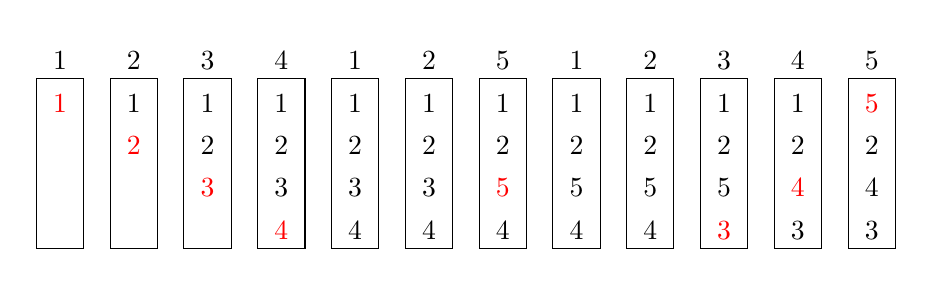
\begin{tikzpicture}[
        every node/.style={
          align=center,
          text height=2ex,
          text width=1em
        },
        swapin/.list={
          (2,1),
          (3,2),
          (4,3),
          (5,4),
          (4,7),
          (5,10),
          (4,11),
          (2,12)
        },
      ]
        \matrix (m) [
          matrix of nodes,
          nodes in empty cells,
          column sep=1em,
          column 2/.style={visible on=<2->},
          column 3/.style={visible on=<3->},
          column 4/.style={visible on=<4->},
          column 5/.style={visible on=<5->},
          column 6/.style={visible on=<6->},
          column 7/.style={visible on=<7->},
          column 8/.style={visible on=<8->},
          column 9/.style={visible on=<9->},
          column 10/.style={visible on=<10->},
          column 11/.style={visible on=<11->},
          column 12/.style={visible on=<12->},
        ] {
          1 & 2 & 3 & 4 & 1 & 2 & 5 & 1 & 2 & 3 & 4 & 5 \\
          1 & 1 & 1 & 1 & 1 & 1 & 1 & 1 & 1 & 1 & 1 & 5 \\
            & 2 & 2 & 2 & 2 & 2 & 2 & 2 & 2 & 2 & 2 & 2 \\
            &   & 3 & 3 & 3 & 3 & 5 & 5 & 5 & 5 & 4 & 4 \\
            &   &   & 4 & 4 & 4 & 4 & 4 & 4 & 3 & 3 & 3 \\
        };
        \draw (m-2-1.north west) rectangle (m-5-1.south east);
        \draw (m-2-2.north west) rectangle (m-5-2.south east);
        \draw (m-2-3.north west) rectangle (m-5-3.south east);
        \draw (m-2-4.north west) rectangle (m-5-4.south east);
        \draw (m-2-5.north west) rectangle (m-5-5.south east);
        \draw (m-2-6.north west) rectangle (m-5-6.south east);
        \draw (m-2-7.north west) rectangle (m-5-7.south east);
        \draw (m-2-8.north west) rectangle (m-5-8.south east);
        \draw (m-2-9.north west) rectangle (m-5-9.south east);
        \draw (m-2-10.north west) rectangle (m-5-10.south east);
        \draw (m-2-11.north west) rectangle (m-5-11.south east);
        \draw (m-2-12.north west) rectangle (m-5-12.south east);
      \end{tikzpicture}
    \end{center}

    \begin{flushright}
      \onslide<13->{8 page faults}
    \end{flushright}
  \end{frame}

  \begin{frame}
    \frametitle{Implementing LRU in Hardware Has to Search All Pages}

    You could implement it by keeping a counter for each page

    \vspace{2em}

    For each page reference, save the system clock into the counter

    \vspace{2em}

    For replacement, scan through the pages and find the one with the oldest clock
  \end{frame}

  \begin{frame}
    \frametitle{Implementing LRU in Software is Too Expensive}

    Create a doubly linked list of pages

    \vspace{2em}

    For each page reference, move it to the front of the list

    \vspace{2em}

    For replacement, remove from the back of the list

    \vspace{2em}

    It requires 6 pointer updates for each page reference, and

    \hspace{2em} also creates a high contention bottleneck for multiple processors
  \end{frame}

  \begin{frame}
    \frametitle{Implementing LRU in Practice Isn't Going to Work}

    We settle for approximate LRU

    \hspace{2em} LRU is an approximation of the optimal case anyways

    \vspace{2em}

    There's lots of different tweaks you can do to implement it more efficiently

    \vspace{2em}

    We'll be looking at the clock algorithm, but there's also:

    \hspace{2em} Least Frequently Used (LFU), 2Q, Adaptive Replacement Cache (ARC)
  \end{frame}

  \begin{frame}
    \frametitle{Page Replacement Algorithms Aim to Reduce Page Faults}

    We saw the following:
    \begin{itemize}
      \item Optimal (good for comparison but not realistic)
      \item Random (actually works surprisingly well, avoids the worst case)
      \item FIFO (easy to implement but Bélády's anomaly)
      \item LRU (gets close to optimal but expensive to implement)
    \end{itemize}
  \end{frame}
\end{document}
